\documentclass{article}

\usepackage{graphicx}
\usepackage{amsmath}
\usepackage{amsfonts}
\usepackage{multirow}

%% Key definitions for text elements. USE THEM
\def\secref#1{Sec.~\ref{#1}}
\def\figref#1{Fig.~\ref{#1}}
\def\tabref#1{Tab.~\ref{#1}}
\def\eqref#1{Eq.~(\ref{#1})}
\def\algref#1{Alg.~\ref{#1}}
\def\appref#1{App.~\ref{#1}}

\newcommand\etal{\emph{et al.}}

\usepackage{amsopn}


\newcommand{\bJidx}[1]{\ensuremath{\mathbf{J}^{[#1]}}}
\newcommand{\cose}{\mathrm{cose}}
\newcommand{\bzidx}[1]{\mathbf{z}^{[{#1}]}}
\newcommand{\bxidx}[1]{\mathbf{x}^{[{#1}]}}
\newcommand{\bhidx}[1]{\mathbf{h}^{[{#1}]}}
\newcommand{\bOmegaidx}[1]{\mathbf{\Omega}^{[{#1}]}}
\newcommand{\bSigmaidx}[1]{\mathbf{\Sigma}^{[{#1}]}}
\newcommand{\bHidx}[1]{\mathbf{H}^{[{#1}]}}

\newcommand{\bv}{\mathbf{v}}
\newcommand{\bl}{\mathbf{l}}
\newcommand{\bt}{\mathbf{t}}
\newcommand{\bo}{\mathbf{o}}
\newcommand{\bM}{\mathbf{M}}
\newcommand{\bL}{\mathbf{L}}
\newcommand{\bA}{\mathbf{A}}
\newcommand{\bB}{\mathbf{B}}
\newcommand{\bE}{\mathbf{E}}
\newcommand{\bK}{\mathbf{K}}
\newcommand{\bC}{\mathbf{C}}
\newcommand{\bH}{\mathbf{H}}
\newcommand{\bI}{\mathbf{I}}
\newcommand{\bP}{\mathbf{P}}
\newcommand{\bX}{\mathbf{X}}
\newcommand{\bZ}{\mathbf{Z}}
\newcommand{\bR}{\mathbf{R}}
\newcommand{\bS}{\mathbf{S}}
\newcommand{\bU}{\mathbf{U}}
\newcommand{\bV}{\mathbf{V}}
\newcommand{\bT}{\mathbf{T}}
\newcommand{\bpi}{\mathbf{\pi}}
\newcommand{\btl}{\mathbf{tl}}
\newcommand{\bbr}{\mathbf{br}}


\newcommand{\iD}{\mathbf{D}}
\newcommand{\iN}{\mathbf{N}}
\newcommand{\iI}{\mathbf{I}}

\newcommand\norm[1]{\left\lVert#1\right\rVert}

\newcommand{\bzridx}[1]{\ensuremath{\mathbf{z}^{({#1})}}}
\newcommand{\bxridx}[1]{\mathbf{x}^{({#1})}}
\newcommand{\bhridx}[1]{\mathbf{h}^{({#1})}}

\newcommand{\bJ}{\mathbf{J}}
\newcommand{\bZero}{\mathbf{0}}

\newcommand{\cS}{\mathcal{S}}
\newcommand{\cC}{\mathcal{C}}
\newcommand{\cSM}{\mathcal{SM}}
\newcommand{\cR}{\mathcal{R}}
\newcommand{\cM}{\mathcal{M}}
\newcommand{\cP}{\mathcal{P}}
\newcommand{\cL}{\mathcal{L}}
\newcommand{\cD}{\mathcal{D}}
\newcommand{\range}[3]{#1_{#2:#3}}


\newcommand{\ba}{\mathbf{a}}
\newcommand{\bb}{\mathbf{b}}
\newcommand{\bc}{\mathbf{c}}
\newcommand{\bd}{\mathbf{d}}
\newcommand{\be}{\mathbf{e}}
\newcommand{\ec}{\mathbf{e}}
\newcommand{\bm}{\mathbf{m}}
\newcommand{\bg}{\mathbf{g}}
\newcommand{\Dim}{\mathrm{Dim}}

\newcommand{\bs}{\mathbf{s}}
\newcommand{\bx}{\mathbf{x}}
\newcommand{\by}{\mathbf{y}}
\newcommand{\br}{\mathbf{r}}
\newcommand{\bz}{\mathbf{z}}
\newcommand{\bu}{\mathbf{u}}
\newcommand{\bn}{\mathbf{n}}
\newcommand{\bh}{\mathbf{h}}
\newcommand{\bff}{\mathbf{f}}
\newcommand{\bp}{\mathbf{p}}
\newcommand{\bDelta}{\mathbf{\Delta}}
\newcommand{\bGamma}{\mathbf{\Gamma}}
\newcommand{\bDeltaalpha}{\mathbf{\Delta \alpha}}
\newcommand{\bDeltar}{\mathbf{\Delta r}}
\newcommand{\bDeltax}{\mathbf{\Delta x}}
\newcommand{\bDeltaX}{\mathbf{\Delta X}}
\newcommand{\bDeltat}{\mathbf{\Delta t}}
\newcommand{\bDeltaR}{\mathbf{\Delta R}}
\newcommand{\tTov}{\mathrm{t2v}}
\newcommand{\vTot}{\mathrm{v2t}}

\newcommand{\bO}{\mathbf{O}}

\newcommand{\defeq}{=}


\newcommand{\bmu}{\mathbf{\mu}}
\newcommand{\bnu}{\mathbf{\nu}}
\newcommand{\bSigma}{\mathbf{\Sigma}}
\newcommand{\bOmega}{\mathbf{\Omega}}
\newcommand{\bLambda}{\mathbf{\Lambda}}

\newcommand{\mat}[1]{#1}
\newcommand{\mbf}[1]{\mathbf{#1}}
\newcommand{\defn}[1]{\emph{#1}}

\newcommand{\mysum}{\sum}
\newcommand{\myprod}{\prod}
\newcommand{\eq}{=}
\newcommand{\pv}{\mathrm{P}}
%\newcommand{\implies}{\Rightarrow}
\newcommand{\Parents}{\mathrm{Parents}}
\newcommand{\rj}{\mathrm{j}}
\newcommand{\proj}{\mathrm{proj}}
\DeclareMathOperator*{\argmax}{argmax}
\DeclareMathOperator*{\argmin}{argmin}
\DeclareMathOperator*{\atantwo}{atantwo}

\newcommand{\mR}{\mathbb{R}}
\newcommand{\mN}{\mathbb{N}}
\newcommand{\mC}{\mathbb{C}}



\title{\LARGE \bf Semantic Mapping Pipeline}

\begin{document}
	
	\maketitle	
	
	\begin{figure}[htbp]
		\centering
		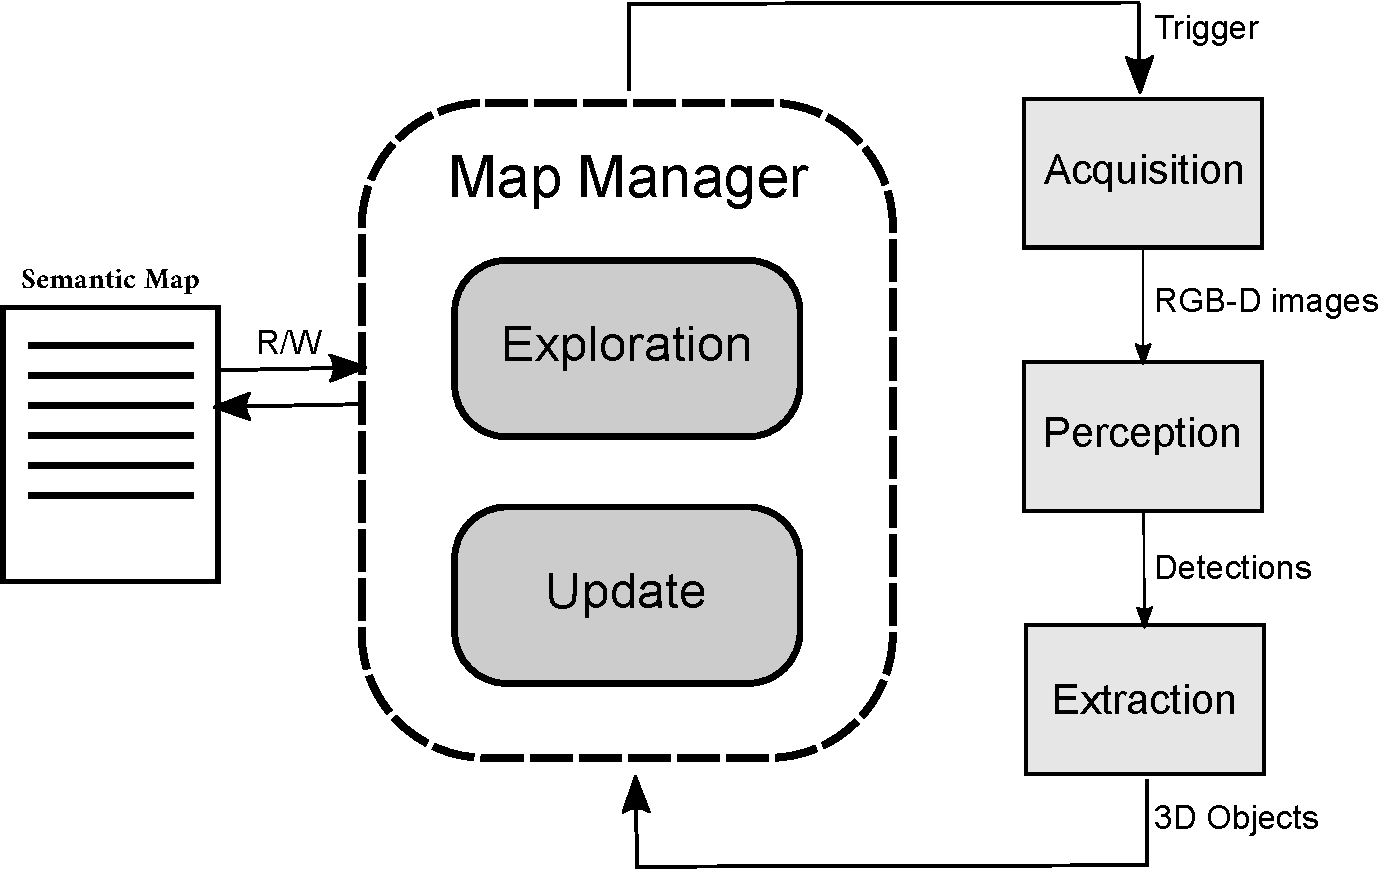
\includegraphics[width=\linewidth]{pics/drawing-crop.pdf}
		\caption{System pipeline.}
		\label{fig:pipeline}
	\end{figure}
	
	\newpage
	\section{Semantic Map}
	
	In our system, a semantic map is a triple:
	
	\begin{equation}
		\cSM = < \cR, \cM, \cP >,
	\end{equation}
	
	\noindent
	with:
	
	\begin{itemize}
		\item $\cR$: reference system
		\item $\cM$: metric information obtained from sensors
		\item $\cP$: predicates compliant with basic concept hierarchy.
	\end{itemize}
	
	\subsection{Global Reference System}	
	
	The reference system is used to express all the elements of the map in a single frame.
	
	\subsection{Metric Map}	
		
	The metric information $\cM$ of the semantic map can be seen as a collection of 3D geometric models:
	
	\begin{equation}
		\cM = \{\bM_1 \cdots \bM_N\},
	\end{equation}
	
	\noindent	
	where each model $\bM_i$ is an entity defined by:
	
	\begin{itemize}
		\item {\bf Pose3D}: $\bX = [ \bR | \bt] \in SE(3)$,
		\item {\bf Size3D}: $\bS = <\bL ,\bU> \in \mathbf{R}^3 $,
		\item {\bf Representation3D}: e.g. a point cloud, a mesh and so on.
	\end{itemize}
	
	The adopted convention is that the pose $\bX$ is assumed to refer to the centroid of the model and that the bounding box $\bS$ is defined by two 3D vectors that specify its "lower" and "upper" corners.
	
	\subsection{Property Map}	
		
	The semantic information $\cP$ contains the assertions about the properties of the objects in $\cM$:
	
	\begin{equation}
	\cP = \{\bP_1 \cdots \bP_N\},
	\end{equation}
	
	\noindent
	where each $\bP_i$ is a set of predicates of $arity = (1 \dots q)$ that are instances of $\bm_i$ (corresponding to the geometrical object $\bM_i$).
	
	\subsection{Interface}
	
	Possible operations on the map are:
	
	\begin{itemize}
		\item query for object: given an object it's possible to check if it's already present in the map
		\item update object: allows to update an object present in the map with a new observation
		\item add object: allows to add an object to the map if it's seen for the first time
		\item render map: builds a 3d model from the collection of objects, this function can be used for navigation and visualization.
		\item serialize/deserialize: these functions allow to save a map on disk and to load it for later use.
	\end{itemize}
	
	\section{Map Manager}
	
	The map manager has the task of incrementally update the semantic map with new observations coming from sensors. The update of the map can be done by registering a local frame with the global model. Once objects refer to the same global frame, data association can be performed to find correspondences between local and global map and update the global map accordingly.
	
	Given the above definition of semantic map, let 
	
	\begin{equation}
		\bE_i \eq < \bM_i,\bP_i >
	\end{equation}
	
	\noindent
	denote the $i^{th}$ element of $\cSM$, where: $\bM_i \in \cM$ is the metric component (expressed in $\cR$) and $\bP_i \in \cP$ the semantic properties. 
	
	Depending on $\cR$, we consider two different maps. The global map $\cSM^G_t = < \cR^G, \cM^G, \cP^G >$  is the collection of elements $\{ \bE_1^G \dots \bE_N^G \}$ referred to the global reference frame at time $t$. While, the local map $\cSM^L_t = < \cR^L, \cM^L, \cP^L >$ is the collection of elements $\{ \bE_1^L \dots \bE_M^L \}$ referred to the robot reference frame at time $t$. 
	
	This allows us to give a definition of correspondence between objects in the two maps. Namely, the $k$-th correspondence
	 
	\begin{equation}
		\bc^{i,j}_k \eq <\bE_i^G,\bE_j^L> 
	\end{equation}
	
	\noindent
	establishes that the $j^{th}$ element $\bE_j^L$ in the local map is the "closest" (w.r.t. a similarity measure, see below) to the $i^{th}$ element $\bE_i^G$ in the global map.
	
	\subsection{Matching} 
	
	{\bf Problem: }	Finding the set of correspondences $\cC_t = \{\bc_1 \dots \bc_K\}$ that states which elements in the global map $\cM^G$ correspond to the one observed in the local map $\cM^L$. This correspondence is evaluated through a similarity measure $d(\bE_i^G,\bE_j^L)$. Thus, computing a correspondence $\bc^{i,j}_k$ consists in finding the element $\bE_j^\star$ that satisfies:
	
	\begin{equation}
		\bE_j^\star = \argmin_{\bE_j} \, d(\bE_i^G,\bE_j^L)
	\end{equation}
		
	\noindent
	{\bf Input: }
	\begin{itemize}
		\item {\bf Global Map}: $\cSM^G_t$
		\item {\bf Local Map}: $\cSM^L_t$
	\end{itemize}
	\noindent
	{\bf Output: }
	\begin{itemize}
		\item {\bf Correspondences}: $\cC_t$		
	\end{itemize}
	\noindent
	{\bf Approaches: }
	\begin{itemize}
		\item brute force
		\item kd-trees
		\item neural networks
	\end{itemize}
	\noindent
	{\bf Remarks: }
	Usually, similarity is computed through euclidean distance. In our problem, we leverage also semantic information. In a simulated environment, the knowledge of the semantic class is perfect. In real world scenarios, object detectors return a probability distribution over semantic labels. In the first case, the corresponding object is the closest one with the same type. In the second case, euclidean distance could be weighted with class probabilities to represent a form of similarity measure.
		
		
%	\begin{table}
%		\begin{center}
%			\begin{tabular}{|r|l|}
%				\multicolumn{2}{c}{\bf Data Association} \\
%				\hline
%				\multirow{2}{*}{\bf Input:} & local map \\
%				& global map\\ \hline
%				{\bf Output:} & correspondences \\ \hline
%				\multirow{3}{*}{\bf Approaches:} & brute-force \\
%				& kd-trees \\
%				& neural networks\\
%				\hline 
%			\end{tabular}
%		\end{center}
%		\caption{Data association.}
%		\label{tab:assoc}
%	\end{table}
	
	\subsection{Update} 
	
	{\bf Problem: } Integrating incoming information from local map into global map. Steps: for each object in local map check if it's already been seen, yes: merge, no: add to map. 
	
	\noindent
	{\bf Input: }
	\begin{itemize}
		\item {\bf Global Map}: $\cSM_t^G$
		\item {\bf Local Map}: $\cSM_t^L$
		\item {\bf Correspondences}: $\cC_t$		
	\end{itemize}
	\noindent
	{\bf Output: }
	\begin{itemize}
		\item {\bf Updated Global Map}: $\cM_{t+1}^G$
	\end{itemize}
	\noindent
	{\bf Approaches: }
	\begin{itemize}
		\item vanilla
		\item age-based
	\end{itemize}
	\noindent
	{\bf Remarks: } This strategy may fail in case of false positives returned by data association. Possible solution:  aging scheme.
	
		
	\section{Action}
	
	\subsection{Exploration} the exploration module has the task of navigating the robot in a way to improve its current knowledge of the environment. 
	
	\subsection{Active Vision} based on the current belief of the problem state, i.e. map and robot pose, and computes a goal pose that maximizes a cost function based on different criteria, e.g., time, space, information gain, human-in-the-loop.
		
	\section{Perception}

	The perception module takes every frame coming from the RGB-D camera and has to tell which objects are seen by the robot. This information will be passed to the map manager so to update the robot knowledge of the environment.
		
	\begin{itemize}
		\item {\bf Image domain}: $\bOmega = \{(u,v) \in \mN^2 \mid u \in [0,height], v \in [0,width]\}$
		\item {\bf RGB domain}: $\bGamma = \{(r,g,b) \in \mN^3 \mid r \in [0,255], g \in [0,255], b \in [0,255]\}$
		\item {\bf Depth domain}: $\bDelta = \{ d \in \mR \mid d \in [0,1]\}$
		\item {\bf Label domain}: $\bLambda = \{ l \in \mN \mid l \in [0,N]\}$
		\item {\bf Pixel}: $\bx \in \bOmega$
		\item {\bf RGB image}: $I : \bOmega \rightarrow \bGamma \implies \bx \rightarrow I(\bx)$
		\item {\bf Depth image}: $D : \bOmega \rightarrow \bDelta \implies \bx \rightarrow D(\bx)$
		\item {\bf Label image}: $L : \bOmega \rightarrow \bLambda \implies \bx \rightarrow L(\bx)$
	\end{itemize}
	
	\subsection{Filtering}
	
	{\bf Problem: } Decide which frame to consider.

	\noindent
	{\bf Input: }
	\begin{itemize}
		\item {\bf RGB Image}: $I$
		\item {\bf Depth Image}: $D$
	\end{itemize}
	\noindent
	{\bf Output: }
	\begin{itemize}
		\item {\bf Trigger}: $t = \{0,1\}$
	\end{itemize}
	\noindent
	{\bf Approaches: }
	\begin{itemize}
		\item \dots
	\end{itemize}
	\noindent
	{\bf Remarks: } \dots
	
	\subsection{Recognition}			
	 
	{\bf Problem: } Finding instances of known class objects in the input image. More formally, given an RGB image $I$ and a set of semantic labels $\cL = \{ l_1 \dots l_N \}$, computes an assignment $L(\bx)$ of labels $l_i$ to each image pixel $\bx$.
	
	\noindent
	{\bf Input: }
	\begin{itemize}
		\item {\bf RGB Image}: $I$
		\item {\bf Semantic Labels}: $\cL$
	\end{itemize}
	\noindent
	{\bf Output: }
	\begin{itemize}
		\item {\bf Label Image}: $L$
	\end{itemize}
	\noindent
	{\bf Approaches: }
	\begin{itemize}
		\item appearance (all computer vision approaches)
		\item geometry (3d object recognition)
	\end{itemize}
	\noindent
	{\bf Remarks: } In a simulated environment it's possible to execute this task by performing only geometrical computations, since one knows the pose of the objects and the robot in the world \dots
	
	\subsection{Extraction}
	
	{\bf Problem: } Building local map from the output of recognition. The first step is to group together pixels with the same semantic label $l_i$. Next, with the depth image $D$, it's possible to recover the 3D position of each image pixel. From this information, the object pose and its size can be inferred, so to build an object:
	
	\begin{equation}
	 \bO = < \bT, \bX, \bS > 
	\end{equation}
	
	\noindent
	{\bf Input: }
	\begin{itemize}
		\item {\bf Label Image}: $L$
		\item {\bf Depth Image}: $D$
	\end{itemize}
	\noindent
	{\bf Output: }
	\begin{itemize}
		\item {\bf Local Map}: $\cM^L = \{ \bO_j^L \}$
	\end{itemize}
	\noindent
	{\bf Approaches: }
	\begin{itemize}
		\item depend on the recognition module
	\end{itemize}
	\noindent
	{\bf Remarks: } \dots
	
\end{document}